\documentclass{article}
\usepackage[none]{hyphenat}
\usepackage{graphicx}

\graphicspath{ {images/} }
\begin{document}

	\title{Bootstrap Estimation of a Non-Parametric Information Divergence Measure}
	\author { \\
		\small Arizona State University}
	\date{}
	\maketitle

%----------------------------------------------------------------------------
	\begin{abstract}
		
		This work details the bootstrap estimation of a non-parametric information divergence measure - the $D_p$ divergence measure - in the context of a binary classification problem. In practice only finite length data sets are available for analysis. To reduce the limitation of finite data size, a bootstrap approach is used to calculate the divergence measure. Monte-Carlo iterations are performed at various sample sizes of the data set, the $D_p$ value is found for each value of sample size, and a power law curve is used to find the asymptotic convergence value of the $D_p$ divergence measure as a function of sample size. The divergence measure can then be used to estimate the Bayes classification error rate. This method is applied to several data sets, and the Bayes error rate is calculated from the $D_p$ divergence.
	\end{abstract}

%----------------------------------------------------------------------------
		\section{Introduction}
		\indent Information divergence measures have a wide variety of applications in machine learning, pattern recognition, statistics, and information theory [8]. A common problem in machine learning is the binary classification problem, in which data $x_i\in$ $\mathbf{R^n}$ is assigned a class label $c_i \in \{0,1\}$ according to a classification rule, where class labels $c_0$ and $c_1$ correspond to respective probability distributions $f_0(\textbf{x})$ and $f_1(\textbf{x})$. The Baysian classifier assigns class labels to $x_i$ such that the posterior probability is maximized []. The error rate of this classifier, the Bayes error rate, provides an absolute lower bound on the classification error rate.  Estimating the best achievable classification error rate makes it possible to quantify the usefulness of a feature set or the performance of a classifier [1]. 
		
		Given the two conditional distributions, $f_0(\textbf{x})$ and $f_1(\textbf{x})$, it is possible to write the Bayes error rate in terms of the prior probabilities $p_0$ and $p_1$ as given in [2]:
		%insert bayes error rate equation here
		\begin{equation} E_{Bayes}=\int_{r_1} p_0f_0(\textbf{x}) \,dx + \int_{r_0} p_1f_1(\textbf{x}) \,dx	\end{equation}
		%ADD PROPER LIMITS TO INTEGRAL
		%
		Here, $r_1$ and $r_0$ refer to the region where the corresponding posterior is the larger[5].
		
		
		Direct evaluation of this integral can be quite involved and impractical, as it is challenging to create an exact model for the posterior distributions $f_0(\textbf{x})$ and $f_1(\textbf{x})$. As an alternative to direct evaluation, it is possible to derive bounds for the Bayes error rate.
		
		
		We arrive at an estimate of the Bayes error rate by using expressions that give bounds on the classification error in terms of information divergence measures. However, common methods of estimating the Bayes error rate via divergence measure still require information about the conditional distributions corresponding to both class labels. Therefore the non-parametric divergence measure given in [3], and the Bayes error estimates derived in [2] will be used in this study.     
		
		
		The work is organized as follows: the remainder of Section 1 is devoted to previous work, Section 2 provides a description of the divergence measure used, and its relation to the Bayes error rate and Section 3 introduces the bootstrap sampling method used. In Section 4 we will apply the method to several generated datasets and real world datasets to show that the power law method can successfully be applied to several distributions. In 4.1 we will consider the generated example datasets, and in 4.2 we will perform our analysis on the Pima Indians dataset and the Banknote dataset found in the University of California Irvine machine learning repository [6].
		%%%Revise%%%
		
		%%%Revise%%%
		
		2
		\subsection*{\small Previous Work}	
		
		%Work on other divergence measures
		%work on parametric divergence measures
		%work on non parametric divergence measure
		% work on f divergence
		%
		
		%dp div eequation
%		When $f_0(\textbf{x})$ and $f_1(\textbf{x})$ have a common region of support, the classification error rate is greater than zero.
		
%----------------------------------------------------------------------------
	
	\section{The $D_p$ Divergence Measure}
	%
	\section{Bootstrap Sampling}

	-lowest sub sample size has to be greater than the dimension of the data
	
	
	\section{Results}
	
	\subsection*{\small Uniform Dataset}

	\begin{table}[ht]
	\caption{Uniform Dataset for Bootstrap Analysis of $D_p$}
	\centering % used for centering table
	\begin{tabular}{c c c c c c c c c c} % centered columns (4 columns)
	 %inserts double horizontal lines
	$D_0$ &  &  &  \\ [0.5ex] % inserts table
	%heading
	\hline % inserts single horizontal line
	$\mu_0$ & 0 & 0 & 0 & 0 & 0 & 0 & 0 & 0\\[0.5ex] % inserting body of the table
	$\sigma_0$ & \( \frac{1}{12} \) & \( \frac{1}{12} \) & \( \frac{1}{12} \) & \( \frac{1}{12} \) & \( \frac{1}{12} \) & \( \frac{1}{12} \) & \( \frac{1}{12} \) & \( \frac{1}{12} \) &  \\[2ex]

	$D_1$ & \\ [0.5ex]
	
	\hline
	$\mu_1$ & \( \frac{1}{2} \) & 0 & 0 & 0 & 0 & 0 & 0 & 0\\[0.5ex] % inserting body of the table
	$\sigma_1$ & \( \frac{1}{12} \) & \( \frac{1}{12} \) & \( \frac{1}{12} \) & \( \frac{1}{12} \) & \( \frac{1}{12} \) & \( \frac{1}{12} \) & \( \frac{1}{12} \) & \( \frac{1}{12} \) &  \\ [1ex] % [1ex] adds vertical space
	\hline %inserts single line
	\end{tabular}
	\label{table:nonlin} % is used to refer this table in the text
	\end{table}
	
	\begin{figure}[h!]
		\caption{Asymptotic Convergence of $D_p$ for 8-Dimensional Uniform Data Set, N = 50 trials}
		\centering
		%	\begin{center}
		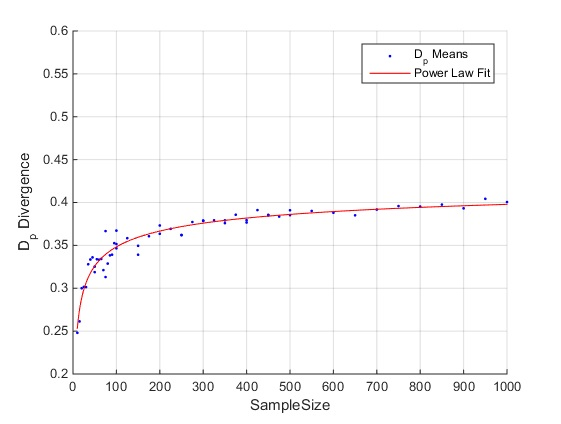
\includegraphics[scale=0.6]{dp_n50_uniform}
		%	\end{center}
	\end{figure}	
	

	\subsection*{\small Gaussian Dataset}
	\begin{table}[!h]
		\caption{Gaussian Dataset for Bootstrap Analysis of $D_p$}
		\centering % used for centering table
		\begin{tabular}{c c c c c c c c c c} % centered columns (4 columns)
			%inserts double horizontal lines
			$D_0$ &  &  &  \\ [0.5ex] % inserts table
			%heading
			\hline % inserts single horizontal line
			$\mu_0$ & 0 & 0 & 0 & 0 & 0 & 0 & 0 & 0\\[0.5ex] % inserting body of the table
			$\sigma_0$ & 1 & 1 & 1 & 1 & 1 & 1 & 1 & 1\\[0.5ex]
			
			$D_1$ & \\ [0.5ex]
			
			\hline
			$\mu_1$ & 0 & 0 & 0 & 0 & 0 & 0 & 0 & 0\\[0.5ex] % inserting body of the table
			$\sigma_1$ & 2.56 & 1 & 1 & 1 & 1 & 1 & 1 & 1\\[0.5ex]
			\hline %inserts single line
		\end{tabular}
		\label{table:nonlin} % is used to refer this table in the text
	\end{table}
			
		\begin{figure}[h!]
			\caption{Asymptotic Convergence of $D_p$ for Gaussian Data Set, N = 50 trials}
			\centering
			%	\begin{center}
			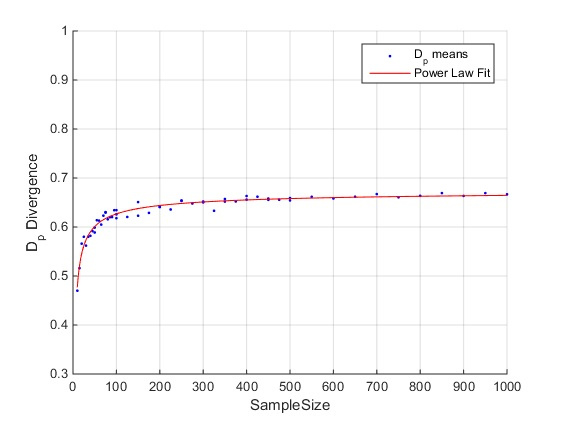
\includegraphics[scale=0.6]{dp_n50_gaussian}
			%	\end{center}
		\end{figure}	
		\newpage
		\subsection*{\small Banknote Dataset}
		The first real world example we consider is the Banknote Authentication Data Set taken from the University of California, Irvine Machine Learning Repository [7]. The 4-dimensional dataset contains data extracted from images of banknotes. The data set consists of a relatively small number of dimensions, and highly separated data, so the convergence is . We note that for a sensitive task such as authenticating banknotes, it should not be surprising to see an asymptotic value for $D_p$ that is close to 1.  
		\begin{figure}[h!]
			\caption{Convergence of $D_p$ for Banknote Authentication Data Set, N = 50 trials}
			\centering
			%	\begin{center}
			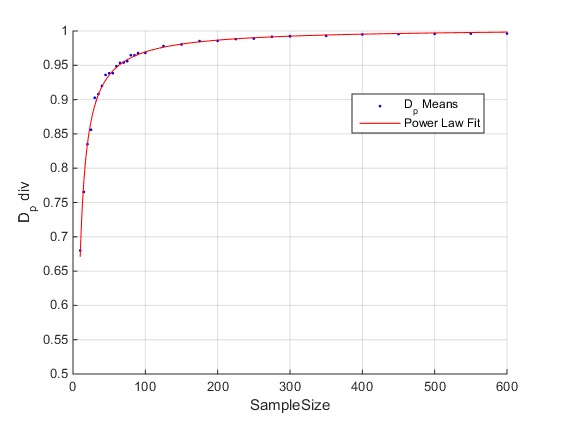
\includegraphics[scale=0.6]{dp_n50_banknote}
			%	\end{center}
		\end{figure}
		
		\newpage
		\subsection*{\small Pima Indians Dataset}
		
		\begin{figure}[!h]
			\caption{Asymptotic Convergence for Pima Indian Data Set, N = 200 trials}
			\centering
			%	\begin{center}
			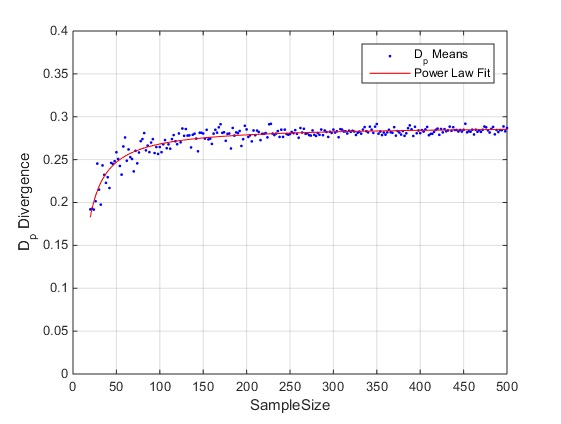
\includegraphics[scale=0.6]{dp_n200_pima}
			%	\end{center}
		\end{figure}	
		
		\begin{figure}[!h]
			\caption{Asymptotic Convergence for Pima Indian Data Set, N = 5000 trials}
			\centering
			%	\begin{center}
			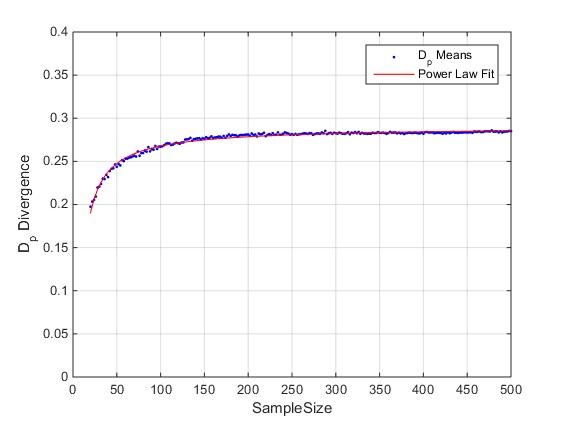
\includegraphics[scale=0.6]{dp_n5000}
			%	\end{center}
		\end{figure}	
		
%		\begin{figure}[!h]
%			\caption{Asymptotic Convergence for Pima Indian Data Set, N = 5000 trials}
%			\centering
%			%	\begin{center}
%			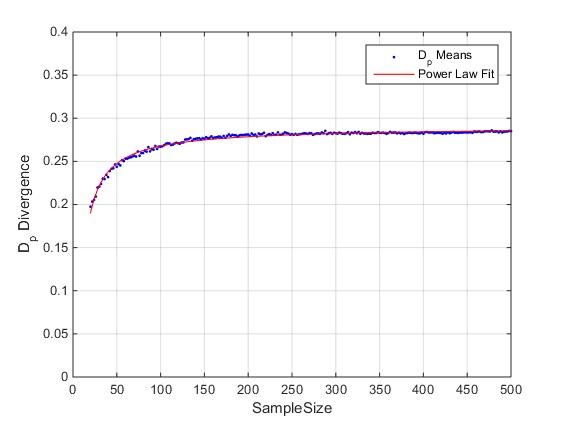
\includegraphics[scale=0.75]{dp_n5000}
%			%	\end{center}
%		\end{figure}	
	\newpage
		\begin{table}[!h]		
			\caption{Bayes Error Rates in Literature for Pima Indians Data Set [4]}
			\begin{center}
				%	\begin{tabular}{||c c c c||} 
				%		\hline
				\begin{tabular}[!h]{ |p{3cm}||p{4cm}|  }
					
					\hline
					Algorithm & Bayes Error Rate (\%) \\ [0.5ex] 
					\hline\hline
					
					 Discrim & 22.50	\\
					 Quadisc &  26.20	\\
					 Logdisc &  22.30	\\
					 SMART  & 23.20	\\
					 ALLOC80 &  30.10	\\
					 K-NN  & 32.40	\\
					 CASTLE &  25.80	\\
					 CART  & 25.50	\\
					 IndCART &  27.10	\\
					 NewID &  28.90	\\
					 AC2 &  27.60	\\
					 Baytree  & 27.10	\\
					 NaiveBay &  26.20	\\
					 CN2  & 28.90	\\
					 C4.5  & 27.00	\\
					 Itrule &  24.50	\\
					 Cal5  & 25.00	\\
					 Kohonen &  27.30	\\
					 DIPOL92 &  22.40	\\
					 Backprob  & 24.80	\\
					 RBF  & 24.30	\\
					 LVQ  & 27.20 	\\
					\textbf{$D_p$ Bootstrap } & \textbf{22.83} \\ 
					\hline 		
				\end{tabular}
			\end{center}
		\end{table}
		
		\begin{table}[!h]		
			\caption{$D_p$ and Bayes Error Rate for the Pima Indian Data Set for Increasing Sample Size, and Increasing Monte-Carlo Iterations}
			\begin{center}
				%	\begin{tabular}{||c c c c||} 
				%		\hline
				\begin{tabular}[!h]{ |p{2cm}||p{2cm}|p{4cm}|p{3cm}|  }
					
					\hline
					Sample Size & Monte-Carlo Iterations & $D_p$ Asymptotic Value (95\% Confidence Interval)& Bayes Error Rate (\%) \\ [0.5ex] 
					\hline\hline
					100	& 50	& 0.2725   (0.245, 0.3)	& 23.90\\
					
					\hline
					
					100	& 200	& 0.2958  (0.265, 0.3267)	& 22.81 \\
					\hline
					
					100	& 5000	& 0.3107  (0.2959, 0.3254)	& 22.13 \\
					
					\hline
					200	& 50	& 0.2946  (0.2732, 0.3161)	& 22.86 \\
					
					\hline
					200	& 200	& 0.3029  (0.288, 0.3178)	& 22.48 \\
					
					\hline
					200	& 5000  & 0.3162  (0.3114, 0.3209)	& 21.88 \\
					
					\hline
					300	& 50	& 0.3118  (0.2827, 0.3409)  & 22.08 \\
					
					\hline
					300	& 200	& 0.3073  (0.2926, 0.3219)	& 22.28 \\
					\hline
					300	& 5000	& 0.3041  (0.3006, 0.3075)	& 22.43 \\ 
					\hline 		
				\end{tabular}
			\end{center}
		\end{table}			
%	\newpage
%		\section{Conclusion}

	\newpage
		\section*{References}
		[1] Hawes, Chad M., and Carey E. Priebe. "A Bootstrap Interval Estimator for Bayes' Classification Error." 2012 IEEE Statistical Signal Processing Workshop, 2012
		\\ [0.5ex]
		\noindent[2] V. Berisha, A. Wisler, A.O. Hero, and A. Spanias, "Empirically Estimable Classification Bounds Based on a Nonparametric Divergence Measure" IEEE Transactions on Signal Processing, vol. 64, no. 3, pp.580-591, Feb. 2016.
		\\ [0.5ex]
		\noindent[3] A. O. Hero, B. Ma, O. Michel, and J. Gorman, “Alpha-divergence for classification, indexing and retrieval,” Communication and Signal Processing Laboratory, Technical Report CSPL-328, U. Mich, 2001
		\\ [0.5ex]
		\noindent [4] K. Tumer, K. (1996) "Estimating the Bayes error rate through classifier combining" in Proceedings of the 13th International Conference on Pattern Recognition, Volume 2, 695–699
		
		Contains the pima indian dataset BERs in table format
		\\ [0.5ex]
		\noindent[5] Tumer, Kagan, and Joydeep Ghosh. "Bayes Error Rate Estimation Using Classifier Ensembles." International Journal of Smart Engineering System Design 5.2 (2003): 95-109.
		\\ [0.5ex]
		
		\noindent[6] Lichman, M. (2013). UCI Machine Learning Repository [http://archive.ics.uci.edu/ml]. Irvine, CA: University of California, School of Information and Computer Science.
		\\ [0.5ex]
		
		\noindent [7] V. Lohweg, “Banknote Authentication Data Set,” 2012. [Online]. Available: https://archive.ics.uci.edu/ml/datasets/banknote+authentication.
	
		\noindent [8] K. Pranesh, and L. Hunter. "On an Information Divergence Measure and Information Inequalities." (n.d.): n. pag. University of Northern British Columbia. 
\end{document}
